\documentclass[../MasterThesis.tex]{subfiles}
\graphicspath{ {./assets/images/} }


%----------------------------------------------------------------------------
%----------------------------------------------------------------------------

\begin{document}
	
	
%
%
%
%
%=======================================================================================================
%
%
%
%
%=======================================================================================================
% CHAPTER: CONCLUSION AND FUTURE WORK
%=======================================================================================================
\newpage
\section{Conclusion} \label{section:conclusion}

In this Chapter, the summary, contributions and limitations are described. After this, opportunities for future work are introduced and examined.






%-------------------------------------------------------------------------------------------------------
\subsection{Summary, Contributions and Limitations} \label{subsection:summary}
% Summarize the key findings and outcomes of the research.


This thesis lays in the field of multimedia processing in real-time, regarding the adjustment of the RGB values of a video with JIT using the Melt framework as a backend. This option was implemented in Codemill's Accurate Player and using WebRTC as a data channel.

For this, background knowledge on colour theory and representation (Chapter \ref{section:theoreticalfoundationofcolour}) and technical background, especially the structure and usage of the Melt framework were given (Chapter \ref{section:technicalbackground}).

The research question consisted of two parts. The first part aimed to evaluate the feasibility of the above described implementation. The implementation confirm that it was achievable. The implementation was described in Chapter~\ref{section:designandimplementation}. This includes a comparison of different Melt filters, to select the most suitable filter for the RGB adjustment. The selected filter is the \texttt{avfilter.colorbalance} filter, which can be used to adjust the RGB values of the highlights, mid tones and shadows individually.


The second part of the research question considers the comparison of video colour grading results with Melt filters, that were applied on different platforms. The compared platforms are the Accurate Player RGB adjustment, that was implemented in this thesis project with the locally installed Melt framework and KDEN Live. This comparison was described in Chapter~\ref{section:experimentalevaluationanddiscussion}.


To evaluate the differences, frames of the different platforms were extracted and compared. 
The colours of those frames have been subtracted from each other using the \textit{grain extract} function in GIMP, to show differences in the colour saturations.


The comparison with the local version of the Melt framework showed the interesting result, that the extracted frames display significant differences, even without the applications of filters. The cause for those differences remains unclear.

The comparison with KDEN Live did not show the same results as the filter application in the Accurate Player either and the results of the colour subtractions lead to the presumption, that KDEN Live is using a different Melt filter for the adjustment of the RGB values.





% Contributions to the Field: Discuss the contributions your thesis makes to the existing body of knowledge in your field. This could include novel insights, methodological advancements, or practical implications of your research.

% Limitations and Future Directions: Acknowledge any limitations or constraints of your study and suggest potential avenues for future research or improvement. This demonstrates a critical reflection on the scope and implications of your work.

% Conclusion: Sum up the overall significance and implications of your research. Reiterate the importance of your findings and their relevance to the broader academic or practical context.

% Closing Remarks: Provide any final thoughts or reflections on the research process, including challenges encountered, lessons learned, or areas for further exploration.

	


	

	
	
	
	





%-------------------------------------------------------------------------------------------------------
\subsection{Future Work} \label{subsection:futurework}
% Suggest possible extensions or improvements to your work.


In this Section, different opportunities for future work are discussed. This includes the implementation of video presets, the application of audio filters, improvements in the user interface and options for advances video processing.


%-------------------------------------------------------------------------------------------------------
\subsubsection*{Video Presets}

Video presets, also known as video filters or video effects, are pre-configured settings or adjustments that can be applied to videos to achieve specific visual styles or effects. 
These presets often include templates for colour grading. 
Video presets are commonly used in video editing software and social media platforms. They provide the user with options to customize their videos easily. 

One example for video presets can be seen in Figure~\ref{figure:app}, where the presets in Adobe Premiere Pro with the \textit{Magic Bullet Looks} plug-in are shown.~\cite{premierepro, magicbullet}

\begin{figure}[H]
	
	\centering
	
	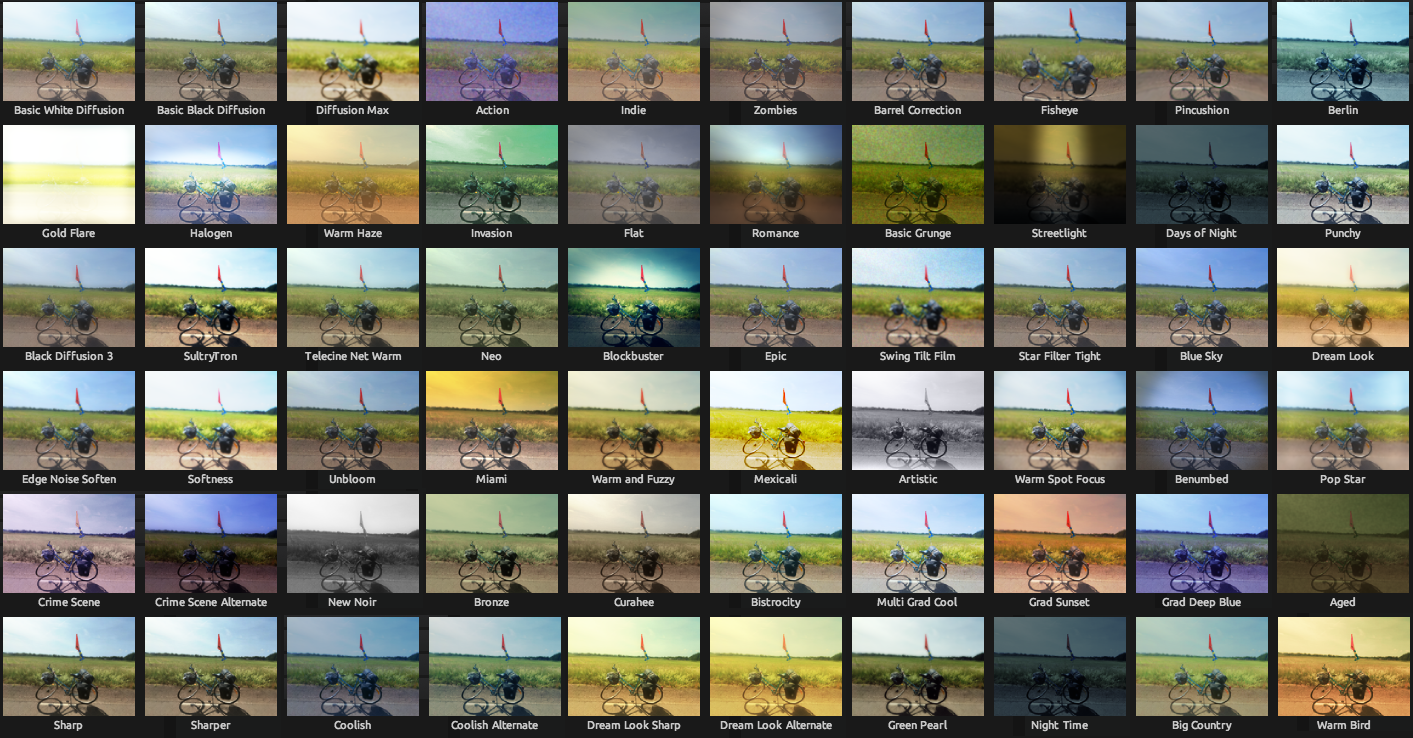
\includegraphics[width=0.99\textwidth]{app.png}
	
	\caption[Presets in Adobe Premiere Pro (\textit{Magic Bullet Looks})]{Presets in Adobe Premiere Pro with the plug-in \textit{Magic Bullet Looks}~\cite{premierepro, magicbullet}}
	\label{figure:app}
	
\end{figure}

Implementing options for the application of those presets is an interesting opportunity for future work. To implement this, different Melt filters can be used or combined. Different options for those Melt filters as video preset filters can be seen in Appendix~\ref{appendix:differentMeltFilter}.













%-------------------------------------------------------------------------------------------------------
\subsubsection*{Advanced Video Processing}

With the implementation of options for advanced video processing tools, other opportunities arise. An online video editing tool with a Melt backend could be implemented. The functionalities could include the cutting of video clips, the application of above described video presets and the manual adjustment of individual video and audio parameters.










%-------------------------------------------------------------------------------------------------------
\subsubsection*{Improvements of the User Interface}

\vspace*{0.5em}

\begin{minipage}{0.38\textwidth}
	Improvements of the user interface can be implemented to make the adjustment of the RGB colours more intuitive. This could involve a preview of the colour, that is being created by adjusting the RGB sliders and then applied to the video. An example for this preview can be seen in Figure~\ref{figure:UI}.
	To decide, which changes in the user inter-
\end{minipage}\begin{minipage}{0.04\textwidth}
	\ 
\end{minipage}\begin{minipage}{0.58\textwidth}
	\begin{figure}[H]
		\begin{center}
			\cutpic{0.3cm}{0.9\textwidth}{ApoADC.png}
			\caption[Example for the colour preview of the RGB sliders.]{Example for the preview of the colour, that is being created by adjusting the RGB sliders and then applied to the video.}
			\label{figure:UI}
		\end{center}
	\end{figure}
	\vfill
\end{minipage}
% \vspace*{1em}

face enhance the usability of the colour adjustment and feel intuitive for the user, extensive testing and user studies could be conducted.




In addition to this, the above described future work opportunities of implementing video presets or an online video editing tool need a design for the user interface as well, to guarantee the usability. 






%-------------------------------------------------------------------------------------------------------
\subsubsection*{Audio filter}

This thesis project focussed on the application of visual filters to a video, especially the adjustment of the RGB values. Aside from this, audio processing plays a role in the processing of videos, too. Similar to the visual content, the audio can enhance the experience and evoke emotions in the viewer. Audio filters can also be used to improve the quality of the recorded audio for example by applying noise suppression or to add context to a scene, by adding fitting surrounding noises. In addition to this, simple aspects including the volume or tone can be modified.
The list of filters on the Melt website contains the available audio filters, too.~\cite{melt}

The implementation of the audio filter integrations is an interesting option for future work. To compare different audio filters, the according sound waves of a track could be read out and compared.









	
	
	
\end{document}